\chapter{Zuivere stoffen en mengsels}\label{ch:g6:pure-substances-and-mixtures}

Op het etiket van een fles mineraalwater staan een stuk of twaalf
opgeloste stoffen, met hun hoeveelheid in milligram per liter. Het water
uit het zuiveringsapparaat van een laboratorium vermeldt er geen enkele.
Beide zijn helder en kleurloos, beide lessen de dorst --- en toch is maar
een van de twee wat een scheikundige zuiver noemt. Dit hoofdstuk geeft
het woord ``zuiver'' zijn precieze betekenis, en laat zien hoe je een
\omterm{def:g6:pure-substances-and-mixtures:pure-substance}{zuivere stof} van een \omterm{def:g6:pure-substances-and-mixtures:mixture}{mengsel} onderscheidt zonder iets te proeven.

\begin{recall}
\omterm{def:g2:mixing-and-dissolving:mix}{Mengen} is verschillende dingen bij elkaar doen; een vaste stof die in
water \omterm{def:g2:mixing-and-dissolving:dissolve}{oplost}, laat de vloeistof helder, en die heldere vloeistof is een
oplossing (\cref{ch:g2:mixing-and-dissolving}). \omterm{def:g6:pure-substances-and-mixtures:mixture}{Mengsels} kun je uit
elkaar halen door \omterm{def:g3:separating-mixtures:sieve}{zeven}, \omterm{def:g3:separating-mixtures:decant}{afschenken}, \omterm{def:g3:separating-mixtures:filter}{filtreren} en \omterm{def:g3:separating-mixtures:evaporate}{indampen}
(\cref{ch:g3:separating-mixtures}). Elk materiaal heeft eigenschappen
die je kunt testen: hard of zacht, doorzichtig of niet, drijft of zinkt
(\cref{ch:g1:materials-around-us}).
\end{recall}

\section{Chemische stoffen en zuivere stoffen}

\begin{definition}[Chemische stof]\label{def:g6:pure-substances-and-mixtures:species}
Een \emph{chemische stof}\index{chemische stof} is één bepaalde soort
stof, met een eigen naam en eigen eigenschappen: water, suiker, zout,
zuurstof, ethanol (de alcohol in wijn), ijzer.
\end{definition}

\begin{definition}[Zuivere stof]\label{def:g6:pure-substances-and-mixtures:pure-substance}
Een \emph{zuivere stof}\index{zuivere stof} bestaat uit één enkele
\omterm{def:g6:pure-substances-and-mixtures:species}{chemische stof} en verder niets: gedestilleerd water, een suikerkristal,
een ring van zuiver goud.
\end{definition}

\begin{definition}[Mengsel]\label{def:g6:pure-substances-and-mixtures:mixture}
Een \emph{mengsel}\index{mengsel} bevat meerdere \omterm{def:g6:pure-substances-and-mixtures:species}{chemische stoffen}.
\omterm{def:g4:air-a-mixture-of-gases:air}{Lucht}, zeewater, mineraalwater, melk, graniet en sinaasappelsap zijn
mengsels.
\end{definition}

\begin{remark}[Zuiver in de omgangstaal]\label{rem:g6:pure-substances-and-mixtures:everyday}
Op een pak ``puur sinaasappelsap'' betekent ``puur'' dat er niets aan
het sap is toegevoegd. Voor een scheikundige is het sap nog steeds een
\omterm{def:g6:pure-substances-and-mixtures:mixture}{mengsel}: water, suikers, zuren, vitamines, kleur- en smaakstoffen, een
heleboel \omterm{def:g6:pure-substances-and-mixtures:species}{chemische stoffen}. ``Zuiver bergwater'' is ook een \omterm{def:g6:pure-substances-and-mixtures:mixture}{mengsel}:
water met opgeloste zouten.
\end{remark}

\begin{omfigure}
\begin{tikzpicture}[font=\small, level distance=1.55cm,
    box/.style={draw=omDef, fill=omDef!6, rounded corners=2pt, align=center,
      inner sep=4pt},
    level 1/.style={sibling distance=7.2cm},
    level 2/.style={sibling distance=3.6cm},
    edge from parent/.style={draw, thick, omDef, ->}]
  \node[box] {materie}
    child {node[box] {zuivere stof\\ \footnotesize één chemische stof}
      child {node[box, draw=black!40, fill=white] {gedestilleerd water,\\ zout, ijzer}}}
    child {node[box] {mengsel\\ \footnotesize meerdere chemische stoffen}
      child {node[box] {homogeen\\ \footnotesize overal hetzelfde}
        child {node[box, draw=black!40, fill=white] {zout water,\\ lucht}}}
      child {node[box] {heterogeen\\ \footnotesize delen zichtbaar}
        child {node[box, draw=black!40, fill=white] {modderwater,\\ graniet}}}};
\end{tikzpicture}

{\small Materie indelen. De onderste vakjes geven van elke soort
voorbeelden.}
\end{omfigure}

\section{Homogene en heterogene mengsels}

\begin{definition}[Homogene en heterogene mengsels]\label{def:g6:pure-substances-and-mixtures:homogeneous}
Een \omterm{def:g6:pure-substances-and-mixtures:mixture}{mengsel} is een \emph{homogeen mengsel}\index{homogeen mengsel} als
je de verschillende delen met het oog niet van elkaar kunt
onderscheiden, zelfs niet met een vergrootglas: het ziet er overal
hetzelfde uit. Het is een \emph{heterogeen mengsel}\index{heterogeen mengsel}
als je minstens twee verschillende delen kunt zien.
\end{definition}

\begin{example}[Vier mengsels]\label{ex:g6:pure-substances-and-mixtures:four}
Zout water en \omterm{def:g4:air-a-mixture-of-gases:air}{lucht} zijn homogeen: je ziet hun delen niet. Olie op water
is heterogeen: twee lagen. Modderwater is heterogeen: er zweven korreltjes
in die \omterm{def:g3:separating-mixtures:decant}{bezinken}. Sinaasappelsap met vruchtvlees is heterogeen: je ziet de
stukjes vruchtvlees.
\end{example}

\begin{omfigure}
\begin{tikzpicture}[font=\small, scale=1.15]
  \pic[transform shape] at (0,0) {beaker={0.7}{omWater!80}};
  \node[anchor=north, align=center] at (0,-0.15) {zout water:\\ homogeen};
  \pic[transform shape] at (2.6,0) {beaker={0.7}{omWater!80}};
  \fill[yellow!55!orange!60] (1.8,1.05) rectangle (3.4,1.4);
  \draw[omGlass, line width=0.7pt] (1.8,1.05) -- (1.8,1.4) (3.4,1.05) -- (3.4,1.4);
  \node[anchor=north, align=center] at (2.6,-0.15) {olie op water:\\ heterogeen};
  \pic[transform shape] at (5.2,0) {beaker={0.7}{brown!25}};
  \foreach \x/\y in {4.6/0.3,4.9/0.7,5.3/0.5,5.6/1.0,5.0/1.1,5.4/0.2,5.8/0.6}
    \fill[brown!65] (\x,\y) circle (0.04);
  \fill[brown!60] (4.4,0) rectangle (6.0,0.12);
  \node[anchor=north, align=center] at (5.2,-0.15) {modderwater:\\ heterogeen};
  \pic[transform shape] at (7.8,0) {beaker={0.7}{orange!45}};
  \foreach \x/\y in {7.3/0.35,7.6/0.8,8.0/0.5,8.3/1.0,7.7/1.15,8.2/0.25,7.45/0.65}
    \fill[orange!80!brown] (\x,\y) ellipse (0.08 and 0.03);
  \node[anchor=north, align=center] at (7.8,-0.15) {sap met vruchtvlees:\\ heterogeen};
\end{tikzpicture}

{\small Eén homogeen en drie \omterm{def:g6:pure-substances-and-mixtures:homogeneous}{heterogene mengsels}.}
\end{omfigure}

\begin{omfigure}
\begin{minipage}[b]{0.48\linewidth}\centering
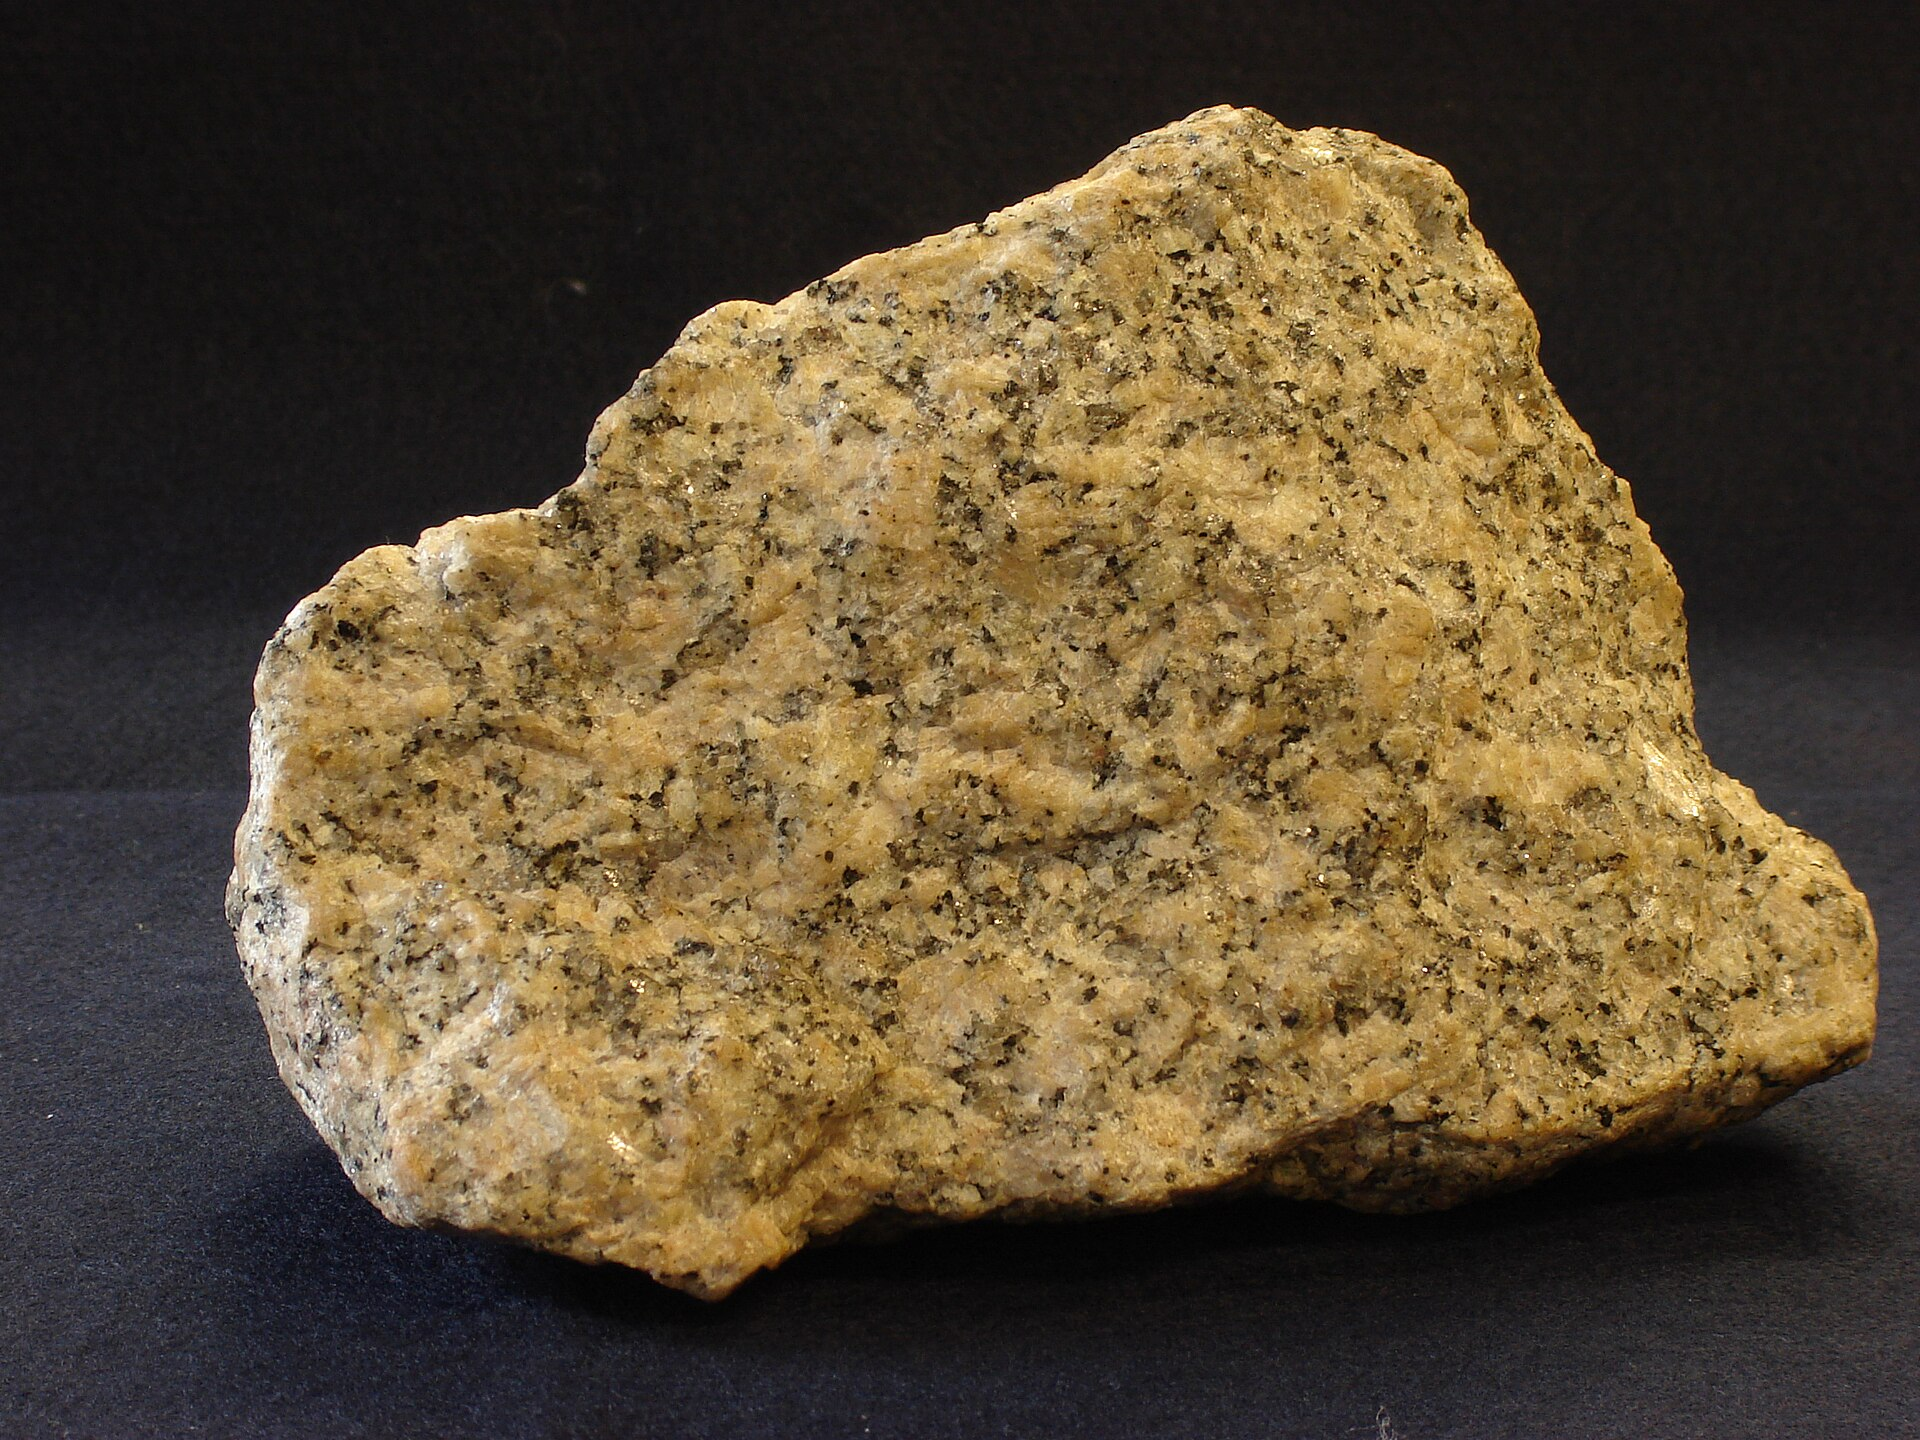
\includegraphics[width=\linewidth,height=4.6cm,keepaspectratio]{images/book1/granite.jpg}

{\small Graniet: je ziet korrels van drie of vier verschillende
mineralen. Een heterogene vaste stof. Foto: Eurico Zimbres, CC BY-SA 2.0 br.}
\end{minipage}\hfill
\begin{minipage}[b]{0.48\linewidth}\centering
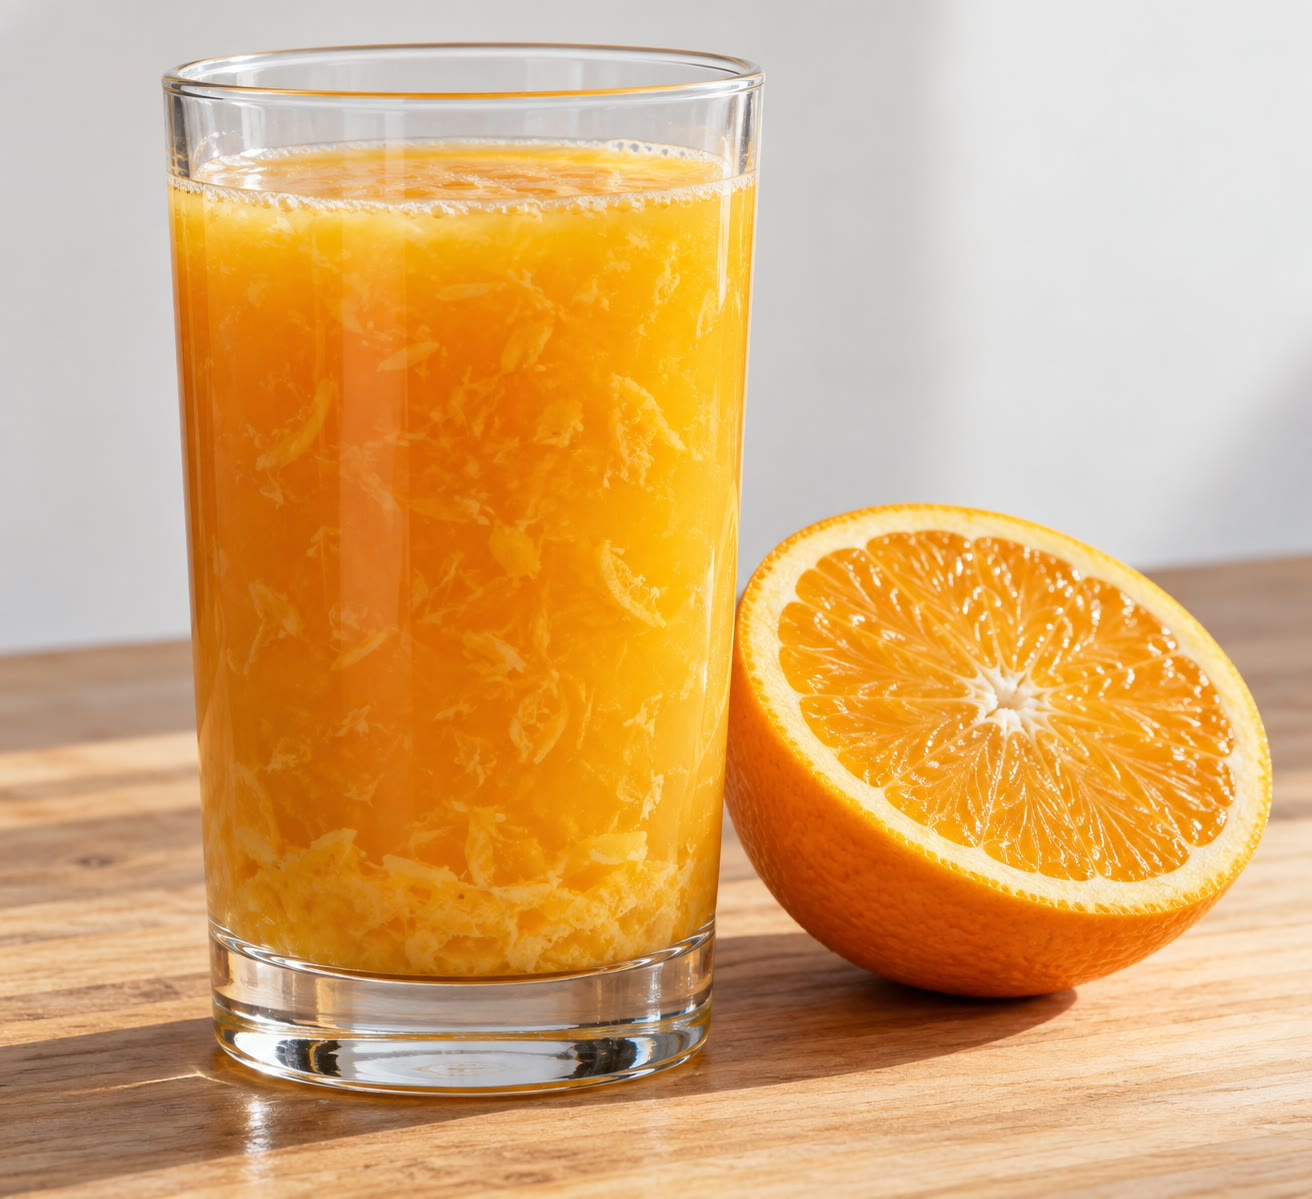
\includegraphics[width=\linewidth,height=4.6cm,keepaspectratio]{images/book1/ai/g6-orange-juice.jpg}

{\small Sinaasappelsap met vruchtvlees: een \omterm{def:g6:pure-substances-and-mixtures:homogeneous}{heterogeen mengsel}.}
\end{minipage}
\end{omfigure}

\begin{remark}[Homogeen betekent niet zuiver]\label{rem:g6:pure-substances-and-mixtures:not-pure}
Zout water ziet er precies zo uit als zuiver water. Kijken is niet
genoeg om een \omterm{def:g6:pure-substances-and-mixtures:pure-substance}{zuivere stof} van een \omterm{def:g6:pure-substances-and-mixtures:homogeneous}{homogeen mengsel} te onderscheiden: we
moeten iets meten.
\end{remark}

\section{Een zuivere stof herkennen aan haar stofconstanten}

\begin{proposition}[Een zuivere stof heeft haar eigen constanten]\label{prop:g6:pure-substances-and-mixtures:constants}
% ledger: mp:water, bp:water, bp:ethanol, mp:ethanol, rho:water, rho:ethanol, mp:NaCl, mp:Fe, rho:Fe
Elke \omterm{def:g6:pure-substances-and-mixtures:pure-substance}{zuivere stof} smelt bij haar eigen vaste temperatuur, kookt bij haar
eigen vaste temperatuur (bij normale druk), en heeft voor een gegeven
volume haar eigen massa, haar dichtheid. Die getallen zijn haar
stofconstanten; het natuurkundeboek legt uit wat ze meten. Voor een paar
\omterm{def:g6:pure-substances-and-mixtures:pure-substance}{zuivere stoffen}:
\begin{center}
\small
\begin{tabular}{lccc}
\hline
\omterm{def:g6:pure-substances-and-mixtures:pure-substance}{zuivere stof} & smeltpunt & kookpunt & massa van \qty{1}{cm^3} \\
\hline
water & \qty{0}{\celsius} & \qty{100}{\celsius} & ongeveer \qty{1.0}{g} \\
ethanol & \qty{-114}{\celsius} & \qty{78}{\celsius} & \qty{0.79}{g} \\
propanon (aceton) & --- & \qty{56}{\celsius} & \qty{0.78}{g} \\
zout (natriumchloride) & \qty{801}{\celsius} & --- & \qty{2.17}{g} \\
ijzer & \qty{1538}{\celsius} & --- & \qty{7.87}{g} \\
\hline
\end{tabular}
\end{center}
% ledger: bp:acetone, rho:acetone, rho:NaCl
\end{proposition}

\begin{proposition}[Een mengsel heeft geen vast kookpunt]\label{prop:g6:pure-substances-and-mixtures:mixture-boils}
Een \omterm{def:g6:pure-substances-and-mixtures:mixture}{mengsel} kookt niet bij één vaste temperatuur: zout water begint iets
boven \qty{100}{\celsius} te koken, en zijn temperatuur blijft stijgen
terwijl het kookt, omdat het water verdwijnt en het achterblijvende zout
steeds geconcentreerder wordt.
\end{proposition}

\begin{method}[Is deze vloeistof zuiver? Welke is het?]\label{met:g6:pure-substances-and-mixtures:identify}
\begin{enumerate}
  \item Verwarm haar, in het laboratorium, en lees de temperatuur af
        terwijl ze kookt.
  \item Blijft de temperatuur vast, dan is de vloeistof waarschijnlijk
        een \omterm{def:g6:pure-substances-and-mixtures:pure-substance}{zuivere stof}: vergelijk die temperatuur met een tabel van
        stofconstanten.
  \item Blijft de temperatuur stijgen, dan is het een \omterm{def:g6:pure-substances-and-mixtures:mixture}{mengsel}.
  \item Bevestig met een tweede constante, bijvoorbeeld de massa van een
        bekend volume.
\end{enumerate}
\end{method}

\begin{inthelab}[Zout water koken]
De docent verwarmt zuiver water en zout water naast elkaar, elk met een
thermometer erin. Het zuivere water kookt bij \qty{100}{\celsius} en
blijft daar zolang het kookt. Het zoute water begint iets boven
\qty{100}{\celsius} te koken, en de thermometer kruipt minuut na minuut
omhoog.
\end{inthelab}

\section{Water, zuiver en niet zuiver}

\begin{example}[Vier soorten water]\label{ex:g6:pure-substances-and-mixtures:waters}
% ledger: sea:salinity
\begin{itemize}
  \item \textbf{Gedestilleerd water}, gemaakt in een laboratorium, is
        bijna precies een \omterm{def:g6:pure-substances-and-mixtures:pure-substance}{zuivere stof}: water en verder niets.
  \item \textbf{Kraanwater} is een \omterm{def:g6:pure-substances-and-mixtures:homogeneous}{homogeen mengsel}: water met kleine
        hoeveelheden opgeloste stoffen (een druppel die op een donker
        bord opdroogt, laat een wit kringetje achter).
  \item \textbf{Mineraalwater} is een \omterm{def:g6:pure-substances-and-mixtures:homogeneous}{homogeen mengsel} waarvan het
        etiket de opgeloste stoffen vermeldt, in milligram per liter.
  \item \textbf{Zeewater} is een \omterm{def:g6:pure-substances-and-mixtures:homogeneous}{homogeen mengsel} met ongeveer
        \qty{35}{g} zouten per kilogram.
\end{itemize}
\end{example}

\begin{omfigure}
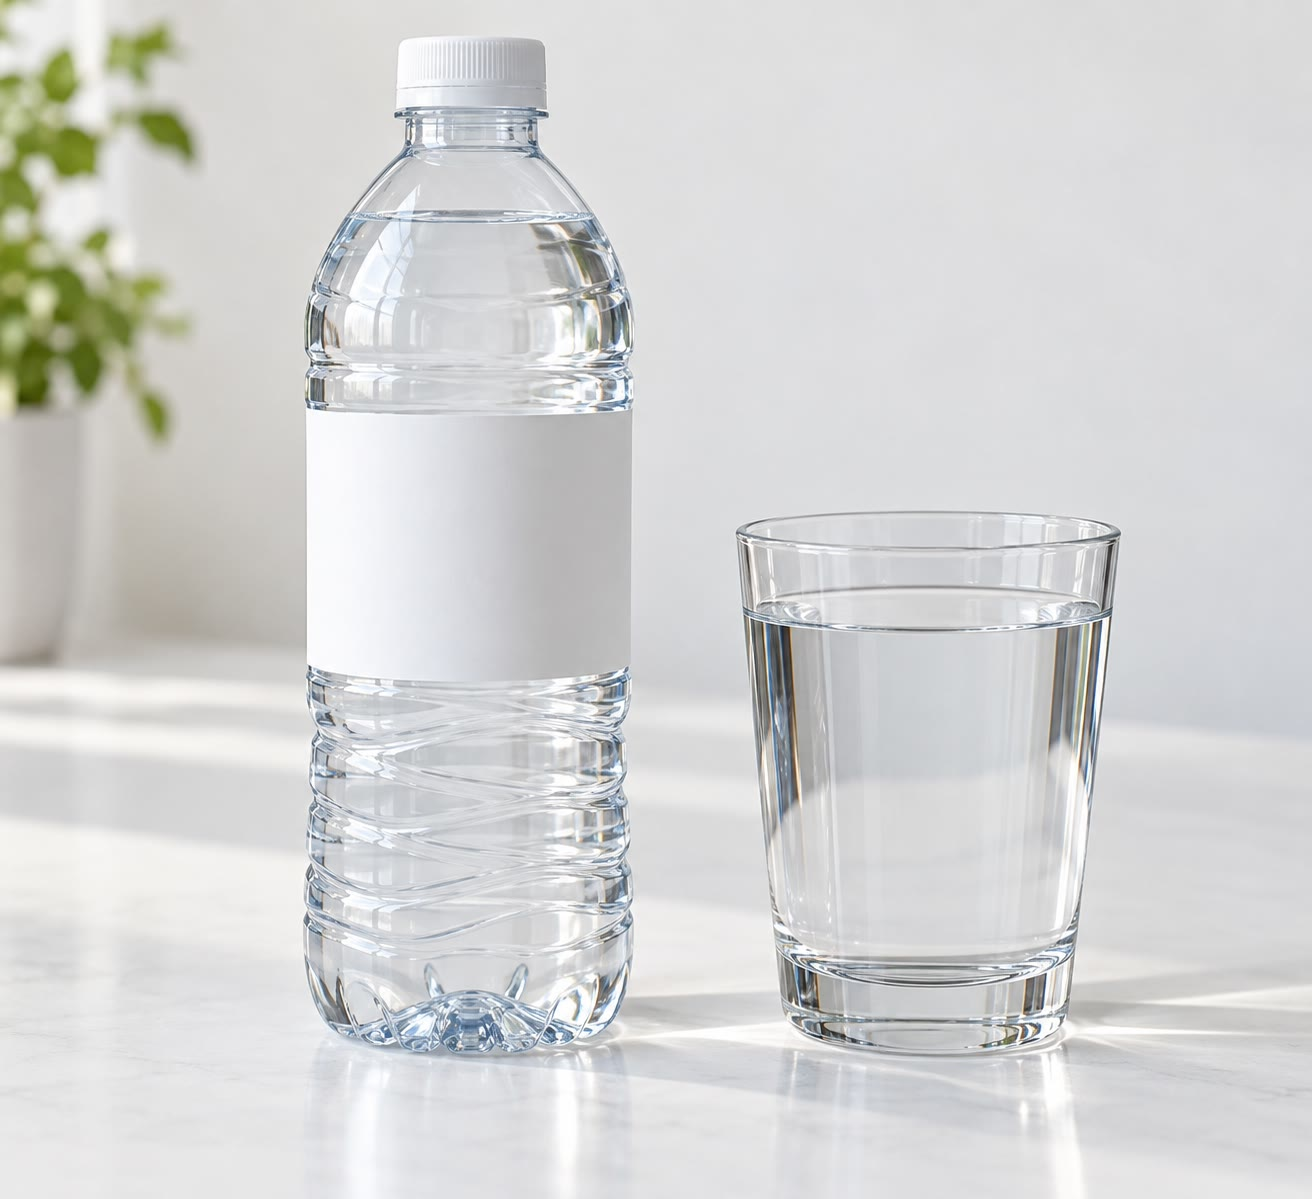
\includegraphics[width=0.5\linewidth]{images/book1/ai/g6-mineral-water.jpg}

{\small Een fles mineraalwater: helder en kleurloos, en toch een
\omterm{def:g6:pure-substances-and-mixtures:mixture}{mengsel}.}
\end{omfigure}

\begin{example}[Het etiket van mineraalwater lezen]\label{ex:g6:pure-substances-and-mixtures:label}
Op een etiket staat: calcium \qty{78}{mg/L}, magnesium \qty{24}{mg/L},
natrium \qty{5}{mg/L}, waterstofcarbonaat \qty{357}{mg/L}, sulfaat
\qty{10}{mg/L}, chloride \qty{4}{mg/L}. (Deze getallen zijn een
voorbeeld.) In één liter zit $78 + 24 + 5 + 357 + 10 + 4 = 478$\,mg
opgeloste stoffen, ongeveer een halve gram: piepklein naast de
\qty{1000}{g} water, maar genoeg om er een \omterm{def:g6:pure-substances-and-mixtures:mixture}{mengsel} van te maken.
\end{example}

\section{Oefeningen}

\begin{exercise}[$\star$]\label{exo:g6:pure-substances-and-mixtures:1}
\omterm{def:g6:pure-substances-and-mixtures:pure-substance}{Zuivere stof} of \omterm{def:g6:pure-substances-and-mixtures:mixture}{mengsel}? Gedestilleerd water, \omterm{def:g4:air-a-mixture-of-gases:air}{lucht}, zeewater, een blok
zuiver ijzer, melk, een suikerkristal.
\end{exercise}

\begin{exercise}[$\star$]\label{exo:g6:pure-substances-and-mixtures:2}
Homogeen of heterogeen? Zout water, graniet, olie op water, kraanwater,
muesli.
\end{exercise}

\begin{exercise}[$\star$]\label{exo:g6:pure-substances-and-mixtures:3}
Wat is een \omterm{def:g6:pure-substances-and-mixtures:species}{chemische stof}? Geef drie voorbeelden.
\end{exercise}

\begin{exercise}[$\star$]\label{exo:g6:pure-substances-and-mixtures:4}
Een vloeistof kookt bij \qty{78}{\celsius}, en haar temperatuur blijft
\qty{78}{\celsius} zolang ze kookt. Gebruik de tabel van stofconstanten
om te bedenken wat het is.
\end{exercise}

\begin{exercise}[$\star$]\label{exo:g6:pure-substances-and-mixtures:5}
Waarom is ``puur sinaasappelsap'' voor een scheikundige geen \omterm{def:g6:pure-substances-and-mixtures:pure-substance}{zuivere
stof}?
\end{exercise}

\begin{exercise}[$\star\star$]\label{exo:g6:pure-substances-and-mixtures:6}
Een vloeistof begint te koken bij \qty{100.5}{\celsius} en haar
temperatuur stijgt terwijl ze kookt. Is het een \omterm{def:g6:pure-substances-and-mixtures:pure-substance}{zuivere stof}? Wat zou het
kunnen zijn?
\end{exercise}

\begin{exercise}[$\star\star$]\label{exo:g6:pure-substances-and-mixtures:7}
Kijk naar de figuur van de vier bekerglazen. In welk bekerglas kan een
filter de delen van het \omterm{def:g6:pure-substances-and-mixtures:mixture}{mengsel} scheiden? In welk bekerglas niet?
\end{exercise}

\begin{exercise}[$\star\star$]\label{exo:g6:pure-substances-and-mixtures:8}
Een metalen kubus met een volume van \qty{10}{cm^3} heeft een massa van
\qty{78.7}{g}. Wat is de massa van \qty{1}{cm^3}? Welk metaal uit de
tabel zou het kunnen zijn?
\end{exercise}

\begin{exercise}[$\star\star$]\label{exo:g6:pure-substances-and-mixtures:9}
Welk percentage van de opgeloste massa is waterstofcarbonaat, volgens het
etiket van het voorbeeld? Rond af op een geheel getal.
\end{exercise}

\begin{exercise}[$\star\star$]\label{exo:g6:pure-substances-and-mixtures:10}
Zeewater bevat ongeveer \qty{35}{g} zouten per kilogram. Hoeveel zout zit
er in een emmer met \qty{2}{kg} zeewater? Welk percentage van de massa
van zeewater is zout?
\end{exercise}

\begin{exercise}[$\star\star\star$]\label{exo:g6:pure-substances-and-mixtures:11}
Twee heldere, kleurloze vloeistoffen zien er precies hetzelfde uit.
Beschrijf twee metingen, uitgevoerd in een laboratorium, die laten zien
of het om dezelfde \omterm{def:g6:pure-substances-and-mixtures:pure-substance}{zuivere stof} gaat.
\end{exercise}

\begin{exercise}[$\star\star\star$]\label{exo:g6:pure-substances-and-mixtures:12}
Een \omterm{def:g6:pure-substances-and-mixtures:mixture}{mengsel} bestaat uit \qty{90}{g} water en \qty{10}{g} ethanol. Welk
percentage van de massa is ethanol? Kun je het met de tabel van
stofconstanten herkennen? Leg uit.
\end{exercise}

\section{Probleem: Drie kleurloze vloeistoffen}

\begin{problem}[{Weekendprobleem --- drie flessen zonder etiket met een
heldere, kleurloze vloeistof, en de metingen die ze onderscheiden}]
\label{pb:g6:pure-substances-and-mixtures:1}
% ledger: bp:water, bp:ethanol, rho:water, rho:ethanol, rho:seawater, sea:salinity
Een laboratoriumassistent vindt drie flessen, A, B en C, waarvan de
etiketten zijn losgeraakt. Alle drie bevatten een heldere, kleurloze
vloeistof. Het laboratorium gebruikt maar drie zulke vloeistoffen:
gedestilleerd water, ethanol, en zeewater dat van een excursie is
meegenomen. De assistent doet drie soorten metingen, in het
laboratorium.

\medskip
\noindent\textbf{Deel I --- Kijken.}
\begin{enumerate}
  \item De drie vloeistoffen zien er precies hetzelfde uit. Kan de
        assistent door te kijken zeggen welke \omterm{def:g6:pure-substances-and-mixtures:pure-substance}{zuivere stoffen} zijn? Leg
        uit.
  \item Als een ervan een \omterm{def:g6:pure-substances-and-mixtures:mixture}{mengsel} is, is dat dan homogeen of heterogeen?
  \item Met welke soort meting kun je laten zien dat een vloeistof een
        \omterm{def:g6:pure-substances-and-mixtures:pure-substance}{zuivere stof} is?
\end{enumerate}

\medskip
\noindent\textbf{Deel II --- Meten.}
Elke vloeistof wordt verwarmd tot ze kookt. Vloeistof A kookt bij
\qty{100}{\celsius} en haar temperatuur blijft daar. Vloeistof B kookt bij
\qty{78}{\celsius} en blijft daar. Vloeistof C begint te koken bij
\qty{100.6}{\celsius}, en haar temperatuur blijft langzaam stijgen.
Daarna wordt van elke vloeistof \qty{50.0}{mL} gewogen: A \qty{49.8}{g}, B
\qty{39.5}{g}, C \qty{51.2}{g}.
\begin{enumerate}[resume]
  \item Welke vloeistoffen zijn \omterm{def:g6:pure-substances-and-mixtures:pure-substance}{zuivere stoffen}? Welke is een \omterm{def:g6:pure-substances-and-mixtures:mixture}{mengsel}?
  \item Geef met de tabel van stofconstanten van dit hoofdstuk de namen
        van vloeistof A en B.
  \item Bereken de massa van \qty{1}{mL} (dat is \qty{1}{cm^3}) van
        elke vloeistof.
  \item Kloppen deze massa's met je antwoord op vraag 5?
  \item Waarom blijft de temperatuur van vloeistof C stijgen terwijl ze
        kookt?
\end{enumerate}

\medskip
\noindent\textbf{Deel III --- Wat zit er in vloeistof C?}
Men laat \qty{100}{mL} van vloeistof C in een schaaltje opdrogen. Als al
het water weg is, blijft er \qty{3.5}{g} witte kristallen over.
\begin{enumerate}[resume]
  \item Wat laat dit residu zien over vloeistof C?
  \item Bereken met de massa van \qty{1}{mL} van C uit vraag 6 de massa
        van \qty{100}{mL} van C, en daarna het percentage van die massa
        dat zout is (op één decimaal).
  \item Zeewater bevat ongeveer \qty{35}{g} zouten per kilogram. Welk
        percentage is dat? Vergelijk met vraag 10.
  \item Trek je conclusie: hoeveel gram zout bevat elke liter van
        vloeistof C, en is vloeistof C het zeewater?
\end{enumerate}
\end{problem}
